\documentclass{article}
\usepackage{graphicx}
\usepackage{amsmath}
\usepackage{amssymb}
\usepackage{mathtools}
\usepackage{datetime}
\usepackage{lipsum}
\graphicspath{{images/}}

\setlength\parindent{0pt}	% no indent for entire document
\setcounter{MaxMatrixCols}{20}

\title{Convolution and Deconvolution}

 
\begin{document}

\begin{titlepage}
\author{Hao Huang}
\date{\today}
\maketitle
\end{titlepage}

\tableofcontents
\newpage

\section{2D Convolution}
\begin{center}
\includegraphics[scale=0.7]{conv}
\end{center}
The blue grid is input image ($4\times 4$), and the green grid is output image ($2\times 2$). The kernel size is $3\times 3$. Stride is 1 and padding is 0. The weight of the kernel at the localization $(i, j)$ is donated as $w_{i, j}$. The value of the image at the location $(i, j)$ is donated as $x_{i,j}$.
The kernel is:
\[
w=
\begin{bmatrix}
w_{0,0} & w_{0,1} & w_{0,0} \\ 
w_{1,0} & w_{1,1} & w_{1,2} \\
w_{2,0} & w_{2,1} & w_{2,2} 
\end{bmatrix}
\]
Rewrite image $X$ as a vector:
$
\begin{bmatrix}
x_{0,0} & x_{0,1} & \dots & x_{3,2} & x_{3,3} 
\end{bmatrix}^T
$.Therefore, convolution can be written as matrix multiplication:
\[
Y=w*X=WX=
\]
\[
\setlength{\arraycolsep}{2pt}
\renewcommand{\arraystretch}{1}
\begin{bmatrix}
w_{0,0} & w_{0,1} & w_{0,2} & 0 & w_{1,0} & w_{1,1} & w_{1,2} & 0 & w_{2,0} & w_{2,1} & w_{2,2} & 0 & 0 & 0 & 0 & 0\\
0 & w_{0,0} & w_{0,1} & w_{0,2} & 0 & w_{1,0} & w_{1,1} & w_{1,2} & 0 & w_{2,0} & w_{2,1} & w_{2,2} & 0 & 0 & 0 & 0\\
0 & 0 & 0 & 0 & w_{0,0} & w_{0,1} & w_{0,2} & 0 & w_{1,0} & w_{1,1} & w_{1,2} & 0  & w_{2,0} & w_{2,1} & w_{2,2} & 0\\
0 & 0 & 0 & 0 & 0 & w_{0,0} & w_{0,1} & w_{0,2} & 0 & w_{1,0} & w_{1,1} & w_{1,2} & 0 & w_{2,0} & w_{2,1} & w_{2,2}\\
\end{bmatrix}
\begin{bmatrix}
x_{0,0}\\ x_{0,1}\\ x_{0,2} \\ x_{0,3} \\ x_{1,0} \\x_{1,1} \\ x_{1,2} \\x_{1,3} \\ x_{2,0}\\ x_{2,1}\\ x_{2,2} \\ x_{2,3} \\ x_{3,0} \\x_{3,1} \\ x_{3,2} \\x_{3,3}
\end{bmatrix}
\]
$W$ is a doubly block circulant matrix (a special case of Toeplitz matrix).
Here we define:
\[
W_0=
\begin{bmatrix}
w_{0,0} & w_{0,1} & w_{0,2} & 0 \\ 0 & w_{0,0} & w_{0,1} & w_{0,2}
\end{bmatrix} \;
W_1=
\begin{bmatrix}
w_{1,0} & w_{1,1} & w_{1,2} & 0 \\ 0 & w_{1,0} & w_{1,1} & w_{1,2}
\end{bmatrix}
\]
\[
W_3=
\begin{bmatrix}
w_{2,0} & w_{2,1} & w_{2,2} & 0 \\ 0 & w_{2,0} & w_{2,1} & w_{2,2}
\end{bmatrix} \;
\bf{0}=
\begin{bmatrix}
0 & 0 & 0 & 0 \\ 0 & 0 & 0 & 0
\end{bmatrix}
\]
$W_0$,$W_1$,$W_2$, and $\bf{0}$ are all Toeplitz matrix. $W$ can be written as:
\[
W=
\begin{bmatrix}
W_0 & W_1 & W_2 & \bf{0} \\ \bf{0} & W_0 & W_1 & W_2
\end{bmatrix}
\]
Therefore, $W$ is a doubly block circulant matrix.

\section{2D Deconvolution}
In the above example, the size of $X$ is $16\times 1$ and the size of $Y$ is $4\times 1$. The dimension of $W$ is $4\times 16$. In order to recover the size of $Y$ to the size of $X$, we just need $W^TY$ (We cannot recover the value of $X$, but just size):
\[
Y^\prime = W^TY = W^T(WX)
\]
If we donate $Y$ as:$
\begin{bmatrix}
y_{0,0} & y_{0,1} & y_{1,0} & y_{1,1}
\end{bmatrix}^T
$, the deconvolution can be written as:
\[
Y^\prime = W^TY = 
\begin{bmatrix}
w_{0,0} & 0 & 0 & 0 \\ w_{0,1} & w_{0,0} & 0 & 0 \\
w_{0,2} & w_{0,1} & 0 & 0 \\ 0 & w_{0,2} & 0 & 0 \\
w_{1,0} & 0 & w_{0,0} & 0 \\ w_{1,1} & w_{1,0} & w_{0,1} & w_{0,0}\\
w_{1,2} & w_{1,1} & w_{0,2} & w_{0,1} \\ 0 & w_{1,2} & 0 & w_{0,2}\\
w_{2,0} & 0 & w_{1,0} & 0 \\ w_{2,1} & w_{2,0} & w_{1,1} & w_{1,0}\\
w_{2,2} & w_{2,1} & w_{1,2} & w_{1,1} \\ 0 & w_{2,2} & 0 & w_{1,2}\\
0 & 0 & w_{2,0} & 0 \\ 0 & 0 & w_{2,1} & w_{2,0} \\
0 & 0 & w_{2,2} & w_{2,1} \\ 0 & 0 & 0 & w_{2,2}
\end{bmatrix}
\begin{bmatrix}
y_{0,0} \\ y_{0,1} \\ y_{1,0} \\ y_{1,1}
\end{bmatrix}
\]
If we rewrite it in convolution format $Y^\prime=w^\prime*Y$, where $w^\prime$ is the top-bottom AND left-right flip of the original filter $w$.
\begin{center}
\includegraphics[scale=0.5]{deconv}
\end{center}
In the above image, the blue grid is $Y$, and the green grid is $Y^\prime$. Stride is 1 and padding is 2.

We can write this process as:
\[
X -> Y = conv(X) -> deconv(Y) -> Y^\prime
\]
To keep $Y^\prime$ has the same size as $X$, we need to add paddings to $conv(X)$. Usually we add 0 paddings to $conv(X)$. There are two common padding strategries:
\begin{enumerate}
\item{Add paddings around an image}
\begin{center}
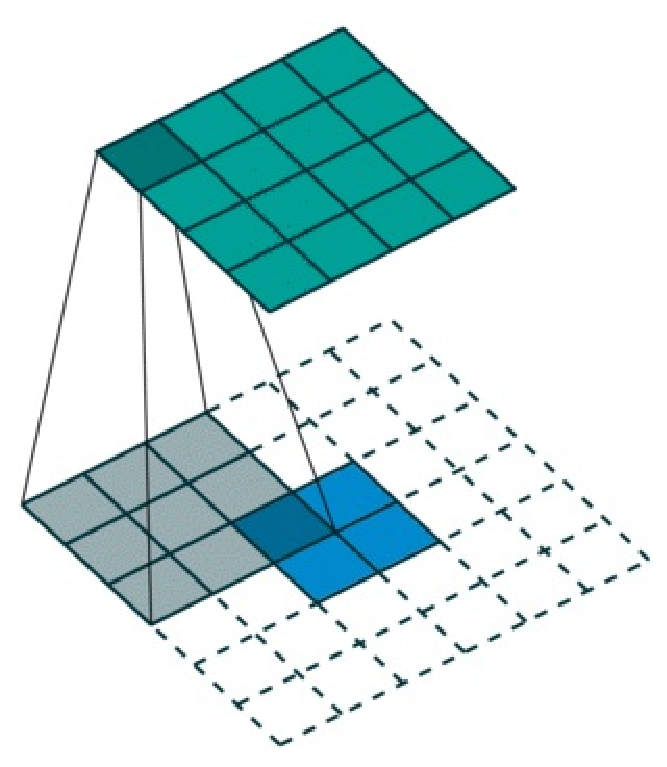
\includegraphics[scale=0.5]{spad}
\end{center}
\item{Add paddings inside an image}
\begin{center}
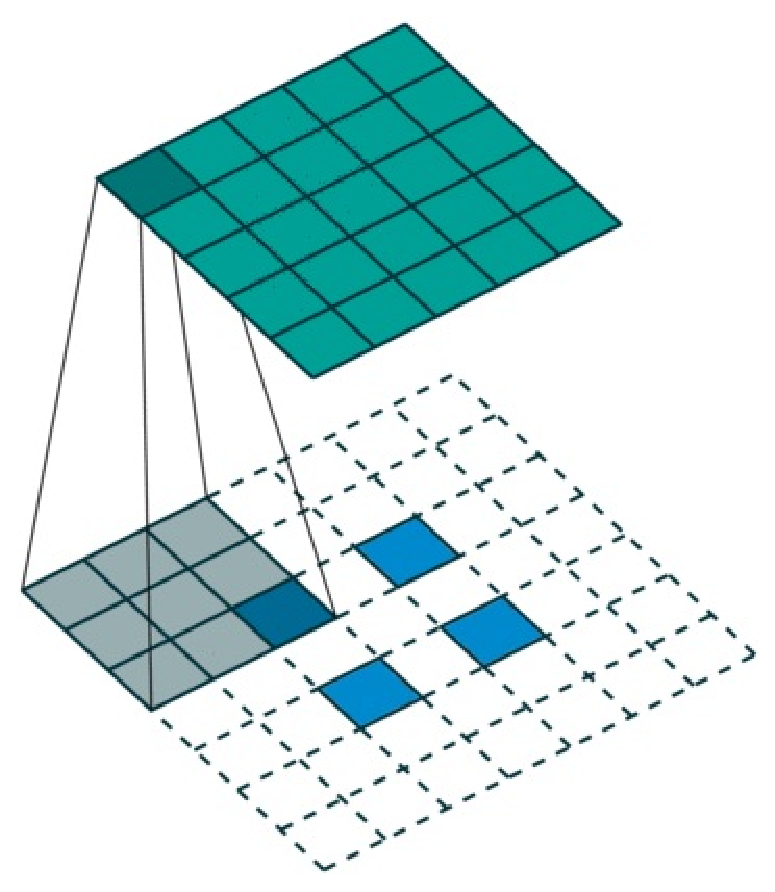
\includegraphics[scale=0.5]{ipad}
\end{center}
\end{enumerate}

These two strategies yield different results. How to choose this two strategies depends on which one can keep the image size.

\end{document}